\chapter{Potentiometer Angle Resolution}\label{potentiometerRes} 
\textbf{Name: Group 630}\\
\textbf{Date: 15/03 - 2016}

\subsubsection{Purpose}
Finding the resolution needed for conversion of potentiometer voltage to angles, along with possible offsets.

\subsubsection{Setup}
\begin{figure}[H]
  \centering
	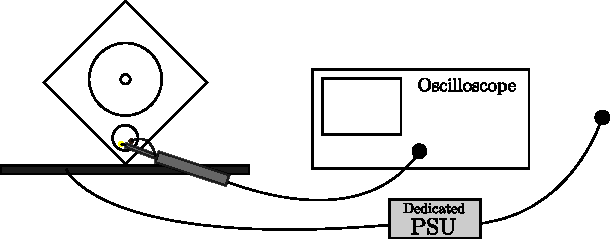
\includegraphics[scale=1]{figures/LabSetupRangeTest.pdf}
	\caption{Setup diagram}
	\label{LabSetupRangeTest}
\end{figure}\vspace{-5mm}

\subsubsection{List of Equipment}
\begin{table}[H]
	\begin{tabular}{|l|l|p{5cm}|}
		\hline%------------------------------------------------------------------------------------------------------------
		\textbf{Instrument}                                  &  \textbf{AAU-no.}  &  \textbf{Type}                       \\
		\hline%------------------------------------------------------------------------------------------------------------
		Oscilloscope                                         &  61604             &  Agilent 54621A		                   \\
		\hline%------------------------------------------------------------------------------------------------------------
		Dedicated Power Supply of Cubli \small{(24 V - 3 A)} &                    &  XP Power, AEB70US24                 \\
		\hline%------------------------------------------------------------------------------------------------------------
		Probe 1:1                                            &  TBD               &  TBD\fxnote{find the probe used}     \\
		\hline%------------------------------------------------------------------------------------------------------------
	\end{tabular}
\end{table}

\subsubsection{Procedure}
\begin{enumerate}
  \item Make the setup with connections as seen on \figref{LabSetupRangeTest}, with ground on brown and signal on yellow of the potentiometer.
  \item Set the oscilloscope on rolling and calibrate so that the full range of the frame movement can be captured on the display.
  \item Balance the frame in upright equilibrium position.
	\item Move the frame to the leftmost position, hold for a brief duration, then move it over to the rightmost position.
	\item Once both the equilibrium, leftmost and rightmost positions are captured on the screen, push the stop-button on the scope, to hold the measurement.
	\item Save the data to the floppy-disk as a CSV-file.
\end{enumerate}

\subsubsection{Results}
\begin{figure}[H] 
	\centering 
	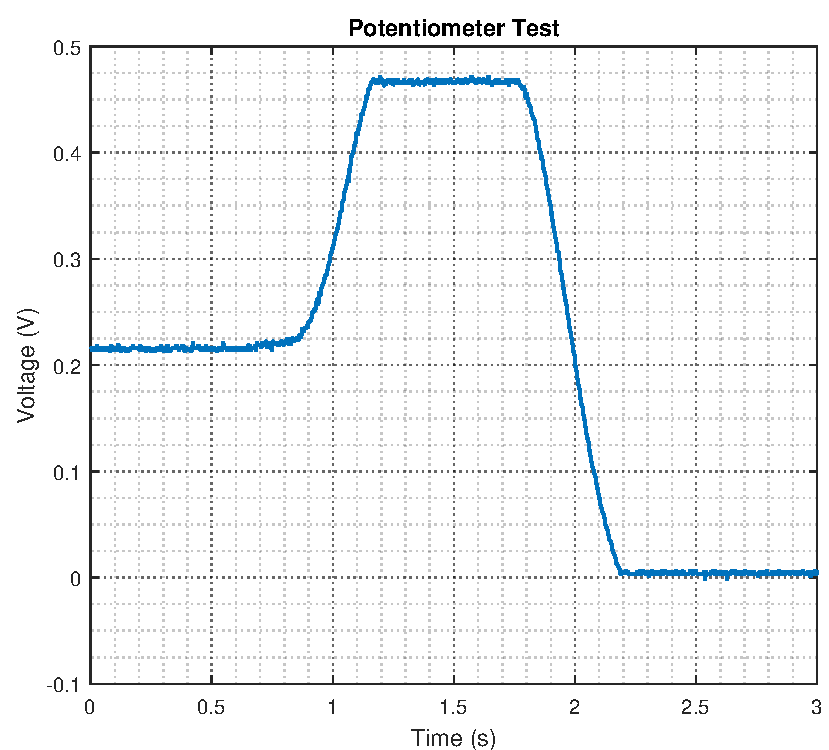
\includegraphics[scale=0.7]{figures/TestPotentiometerResolution}
	\caption{Raw test data plot, Volt over time}
	\label{comparisonRealModel}
\end{figure}